\documentclass[a4paper, 11pt, spanish]{article}
%QUITA IDENTACION
\setlength{\parindent}{0pt}

% ---------------- Paquetes de formato.
\usepackage[spanish]{babel} % Para codificar el texto.
\usepackage[top=70mm, bottom=30mm, left=18mm, right=18mm]{geometry} % Para modificar el tamaño de las hojas.
\usepackage{fancyhdr} % Para poner la institución, dpto y curso arriba.
\usepackage{parallel} % Para escribir en columnas (Poner los integrantes a la derecha).
\usepackage[firstpage=false]{background} % Para poner el logo de la U arriba en todas las páginas.
\usepackage{enumerate} % Para poder enumerar como a), b), etc.
\usepackage[utf8]{inputenc} % Para usar acentos en vez de \'.

% ---------------- Paquetes graficos.
\usepackage{graphicx} % remove the demo option.
\usepackage{tikz}
\usepackage{caption}
\usepackage{subcaption} % Para usar sub-figuras

% ---------------- Paquetes matematicos.
\usepackage{amsmath} % Para poder hacer N^o y se vea bonito.
\usepackage{amsthm} % Fonts matematicos.
\usepackage{amssymb} % Para usar \therefore
\usepackage{commath} % Para usar \abs y \norm

% ---------------- Paquetes 'computines'.
\usepackage{listings} % Para escribir codigo y que se vea bonito.
\usepackage[% Descomentar las opciones a usar.
spanish,
%boxed, % Encierra los algoritmos en un cuadro.
boxruled, % Encierra los algoritmos en un cuadro colocando el titulo al comienzo.
%ruled, % Coloca una linea al comienzo y otra al final del algoritmo. El titulo de este queda al comienzo del algoritmo.
%algoruled, % Lo mismo que el anterior pero mas espaciado.
%tworuled, % Como ruled pero sin una linea al comienzo.
%algochapter, % Los algoritmos se enumeran segun capitulo.
%algopart, % Los algoritmos se enumeran por partes.
%figure, % Los algoritmos son considerados figuras (y por ende salen en \listoffigures).
%linesnumbered, % Enumera las lineas.
longend % Los end son para cada ciclo, por ejemplo endif para los if-else.
]{algorithm2e}

% ---------------- Paquetes miscelaneos.
%\usepackage{lipsum} % Para hacer placeholders.
\usepackage{bohr} % Para dibujar atomos.

% ---------------- Comando mas corto para insertar figuras. Ojo que deben estar guardadas en ./img/
% \fig{name}{width}{height}{caption}
\newcommand{\fig}[4]{%
	\begin{figure}[!htbp]
		\centering
		\includegraphics[width=#2, height=#3]{img/#1}
		\caption{#4}
	\end{figure}
}
% ejemplo:
%\fig{nombre_imagen.png}{10cm}{5cm}{Titulo de la imagen}

%%% Ejemplo para poner dos imagenes juntas, lado a lado

%\begin{figure}[!ht]
%\centering
%\begin{subfigure}{.5\textwidth}
%  \centering
%  \includegraphics[width=10cm, height=8cm]{img/curva0f1.pdf}
%  \caption{Curva de nivel 0 de $F_{1}$.}
%  \label{fig:sub1}
%\end{subfigure}%
%\begin{subfigure}{.5\textwidth}
%  \centering
%  \includegraphics[width=10cm, height=8cm]{img/curva0f2.pdf}
%  \caption{Curva de nivel 0 de $F_{2}$.}
%  \label{fig:sub2}
%\end{subfigure}
%\caption{Curvas de nivel 0 de $F_{1}$ y $F_{2}$}
%\label{fig:test}
%\end{figure}


% ---------------- Comando para hacer itemes
% \Solution{pregunta}{solucion}
\newcommand{\Solution}[2]{%
	\item #1 \vspace{0.2cm}
	\textbf{Soluci\'on:} #2
}
% \Demonstration{pregunta}{demostracion}
\newcommand{\Demonstration}[2]{%
	\item #1 \vspace{0.2cm}
	\begin{proof}
		#2	
	\end{proof}
}

% ---------------- Opciones de algortihm2e
\SetKw{KwRequire}{Require:}

% ---------------- Opciones de background.
\SetBgColor{black}
\SetBgScale{1}
\SetBgOpacity{1}
\SetBgAngle{0}
\SetBgContents{%
	\begin{tikzpicture}[remember picture,overlay]
		\node at (-8.0,0.746\textheight) {\includegraphics[height=18mm,width= 0.155\textwidth]{img/LogoUIngenieria.png}};
	\end{tikzpicture}
}

% ---------------- Creacion de institucion, departamento y curso.
\fancyheadoffset[L]{-2cm}
\fancyhead[L]{\footnotesize{\textbf{\textsf{Universidad de Chile \\ Facultad de Cs. F\'isicas y Matem\'aticas \\ Departamento de F\'isica \\ Métodos Númericos : FI3104-1}}}}
\renewcommand{\headrulewidth}{0pt}
\setlength{\voffset}{-3cm}

\pagestyle{fancy} % Estilo de las páginas

\begin{document}

\pagenumbering{gobble} % Quita el numero de las paginas (y las resetea a 1)

\clearpage

\thispagestyle{fancy}
\vspace*{6.5cm} % Espacio vertical para posicionar bien el título (En una de esas esto se puede optimizar para que no sea tan a la fuerza bruta).

% ---------------- Titulo.
\begin{center}
	\Large{\textbf{\textsf{Informe Tarea 2}}} \\
	\huge{\textbf{\textsf{Algoritmo de Búsqueda de Ceros}}}
\end{center}

\vspace*{7.5cm}

% ---------------- Integrantes, profes, etc.
\begin{Parallel}{1cm}{7.5cm}
	\ParallelRText{%
		\begin{flushright} % Tira el texto hacia la derecha.
			\large{%
				\textsf{%
					\begin{tabular}{rl}
						Alumno: &
							\begin{tabular}[t]{@{}l@{}}
								Bruno Quezada
							\end{tabular} \\
						Profesore: & 
							\begin{tabular}[t]{@{}l@{}}
						 		Valentino González
							\end{tabular} \\
						Auxiliares: &
							\begin{tabular}[t]{@{}l@{}}
								José Vines. \\
								Jou-Hui Ho.
							\end{tabular} \\	 
					\end{tabular} \\
					Fecha: \today
				}
			}
		\end{flushright}
	}
\end{Parallel}

\clearpage

\pagenumbering{arabic} % Numeros de pagina Arabicos (y los resetea a 1)

\newpage

\tableofcontents % Indice. Descomente para usar.
%\listoffigures % Lista de figuras. Descomente para usar.
%\listoftables % Lista de tablas. Descomente para usar.

\newpage
\section{Pregunta 1}
Para esta pregunta se solicita encontrar el largo de un cable entre 2 torres separadas por $20[m]$, con una caída de $7.5[m]$ en su punto medio. La ecuación que modela la forma que adopta el cable es la catenaria definida como $Cat(x,x_0,\alpha) = \frac{\alpha}{2}(e^{\frac{x-x_0}{\alpha}} + e^{-\frac{x-x_0}{\alpha}})$. Para la resolución de este problema es necesario primero encontrar el $\alpha$ que cumpla la condición que baje 7.5 $[metros]$ en su punto medio, esto se hará por medio de la definición de una función auxiliar, la cual se anula en un punto de interés, y se utilizará un algoritmo que busque las raíces de esta función. Una vez encontrado $\alpha$ queda determinada la forma del cable y a través de la integración de $\int_0^{20} \sqrt{Cat'(x,x_0,\alpha)^2 + 1} dx $ se puede determinar su largo.

\subsection{Procedimiento}
Primero es necesario definir una función auxiliar adecuada que al anularse nos permita conocer el valor de $\alpha$ para este caso particular. Se utiliza $f(x,x_0,\alpha) = cat(x_0,x_0,\alpha) - cat(0,x_0,\alpha) + 7.5$ de modo que se anule cuando el cable alcance los $7.5 [m]$ de caída en el punto medio.\\ 
Se construye el método de Newton al cual se le entrega como punto inicial $-5$ y también se implementa el método de la bisección, para este último por inspección $f$ se encuentra el intervalo $[-6,-8]$.
Una vez encontrado $\alpha$ se procede a calcular el largo del cable, esto se logra a través de la integral $\int_0^{20} \sqrt{Cat'(x,x_0,\alpha)^2 + 1} dx $ se estima el valor del largo utilizando la función \textit{scipy.integrate.quad}.

\subsection{Resultados}
El valor de $\alpha$ obtenido corresponde a $-7.667...$ ,para ambos métodos, habiendo diferencias del orden de $\approx 10^{-13}$ entre ambas convergencias. \\
El valor obtenido del largo es $L = 26.09[metros]$. En la figura \ref{catenaria1} se presenta el gráfico de cómo se debe ver el cable entre $0$ y $20 [m]$.\\
Al evauar la función auxiliar en la solución encontrada por la bisección se obtiene $h(\alpha) \approx 10^{-13}$ y por Newton $h(\alpha) = 10^{-15}$.

\begin{figure}[h]
\centering
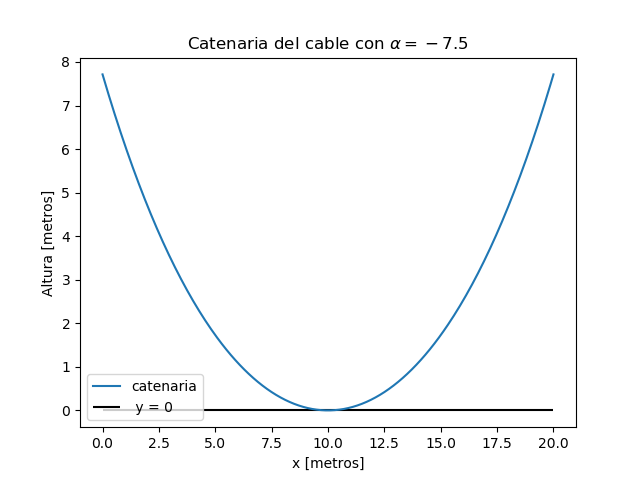
\includegraphics[scale=0.5]{catenaria.png}
\caption{Catenaria que describe la cuerda de largo $L = 26.31 [m]$ } 
\label{catenaria1}
\end{figure} 


\subsection{Conclusiones y Discusi\'on}
En este caso se implementaron dos métodos distintos para encontrar la solución, con el fin de poder compararlos. Ambos algoritmos utilizaron el mismo margen de error para converger de $\epsilon = 10^{-12}$. Es importante recalcar que la comparación jamás puede ser justa, ya que el método de la bisección tiene un intervalo inicial del que no se puede salir el algoritmo, mientras que para el método de Newton solo se entrega un punto inicial. Considerando estas salvedades los tiempos de convergencia de los algoritmos fueron de: Newton $45.2 [\mu s]$ y bisección: $336 [\mu s]$ . y las iteraciones necesarias para converger fueron de: Newton = $6$ y bisección = $41$. Podemos apreciar que la velocidad de convergencia y la cantidad de iteraciones es aplastantemente mejor para Newton, esto se debe a que tiene una velocidad de convergencia cuadrática en comparación con la bisección cuya convergencia es lineal.\\
Como conclusión, es importante conocer bien el algoritmo que se utiliza para la resolución, para poder elegir el más adecuado. En particular, el método de Newton tiene la desventaja de que no es posible utilizarlo en todos los casos debido a que puede converger a otro cero o puede alejarse mucho de la solución, además de exigir que la función sea derivable, en cambio, la bisección sólo necesita que la función sea contína, ya que su convergencia se basa en el teorema del valor intermedio.




\pagebreak
\section{Pregunta 2}

\subsection{Introducci\'on}
En esta pregunta se busca encontrar la región en que las funciones:\\
 $F_1(x,y) = x^4 + y^4 - 15$\\
 $F_2(x,y) = x^3y - xy^3 - \frac{y}{2} - 1.271$\\
\textbf{(RUT:19.133.271-7}) son nulas en forma simultánea. 

\subsection{Procedimiento y Resultados}
En primer lugar, se grafican ambas funciones adaptando el archivo \textit{contourplot.py}. En las figuras \ref{F1} y \ref{F2} se presentan los gráficos de las funciones $F_1$ y $F_2$ respectivamente. Se observa que la región en que F1 se anula corresponde a una curva cerrada, por lo que a través de un cambio de variables es posible parametrizarla. La curva parametrizada queda definida como:\\
 $C(\theta) = (sign(seno(\theta))*\sqrt[4]{15 seno^2(\theta)},sign(cos(\theta))*\sqrt[4]{15 cos^2(\theta)}) $ con $ 0 \leq \theta < 2 \pi$ \\
 
\begin{figure}[h]
\centering
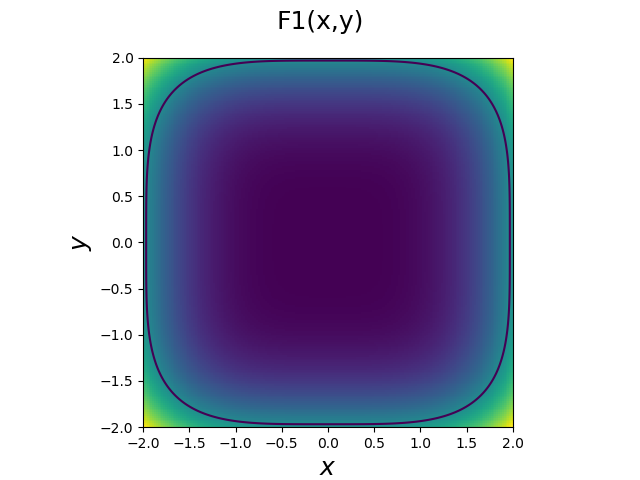
\includegraphics[scale=0.5]{contornoF1.png}
\caption{Contorno de la función $F_1$, con la curva de nivel $F_1 = 0$ en morado} 
\label{F1}
\end{figure} 

\begin{figure}[h]
\centering
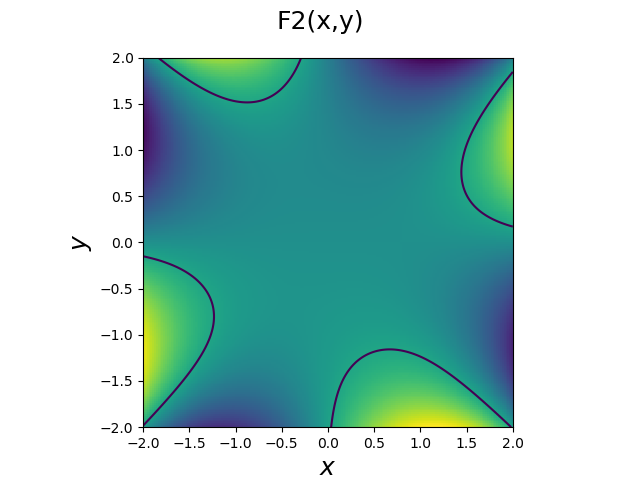
\includegraphics[scale=0.5]{contornoF2.png}
\caption{Contorno de la función $F_2$, con la curva de nivel $F_2 = 0$ en morado} 
\label{F2}
\end{figure} 

La curva parametrizada se presenta en la figura \ref{curva}. Con la parametrización completa se define la función $curva(\theta)$  la cual recorre la curva parametrizada dado un $\theta$. Para encontrar los ceros de $F_2$ primero es necesario estimar los a y b que inicien la bisección de cada cero, para ello es necesario graficar la función $F_2$ a lo largo de la curva, el gráfico se presenta en la figura \ref{cf2}.\\

\begin{figure}[h]
\centering
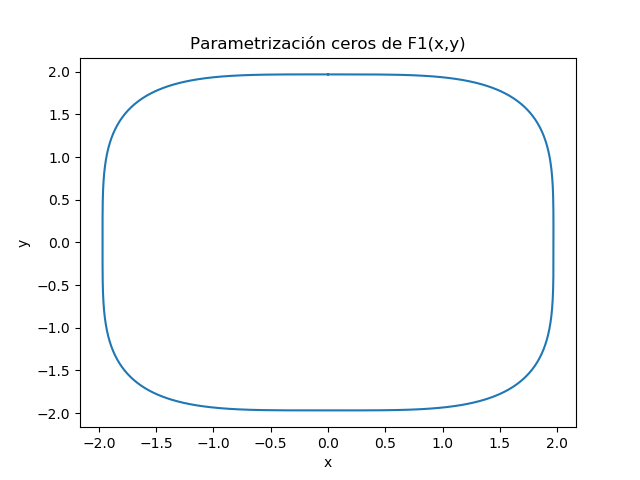
\includegraphics[scale=0.5]{parametrizacion.png}
\caption{Forma de la parametrización de la curva que representa la región con ceros de $F_1$} 
\label{curva}
\end{figure} 

\begin{figure}[h]
\centering
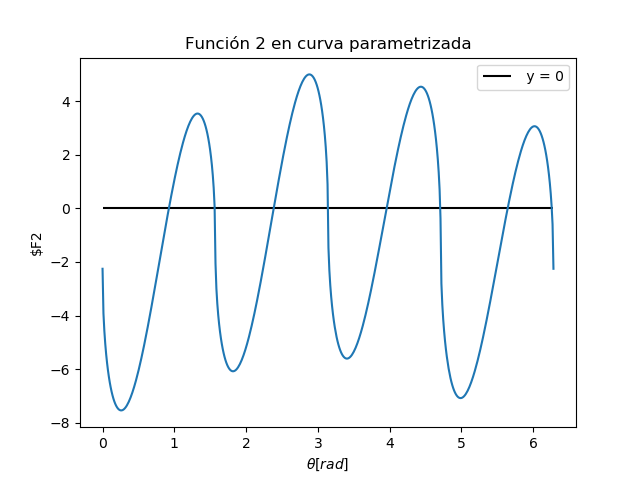
\includegraphics[scale=0.5]{cerosf2.png}
\caption{Función $F_2$ evaluada en la curva parametrizada en azul, recta $y = 0$ en negro} 
\label{cf2}
\end{figure}

Se identifican 8 puntos en donde se anula la función, en la tabla \ref{tab} se definen los a y b para cada cero, con $\theta s$ creciente.\\

\begin{table}[h]
\centering
\caption{Tabla con valores de a y b para cada cero encontrado de la función $F_2$ en la curva parametrizada}
\label{tab}
\begin{tabular}{|c|c|c|}
\hline
\multicolumn{3}{|l|}{\textbf{a y b de cada cero para la $F_2$ parametrizada}} \\ \hline
\multicolumn{1}{|l|}{\textbf{}} & \textbf{a} & \textbf{b} \\ \hline
Cero \#1 & 0,7 & 1,2 \\ \hline
Cero \#2 & 1,4 & 1,7 \\ \hline
Cero \#3 & 2,1 & 2,6 \\ \hline
Cero \#4 & 2,9 & 3,3 \\ \hline
Cero \#5 & 3,7 & 4,1 \\ \hline
Cero \#6 & 4,5 & 4,8 \\ \hline
Cero \#7 & 5,5 & 5,7 \\ \hline
Cero \#8 & 5,9 & 6,27 \\ \hline
\end{tabular}
\end{table}

Se construye la función \textit{biseccion-modificada()} la cual ocupa el algoritmo de la bisección para encontrar los ceros, pero va recorriendo la curva parametrizada. en la figura \ref{ceros} se presentan los valores de la función $F_2$ evaluada en los ceros encontrados.

\begin{figure}[h]
\centering
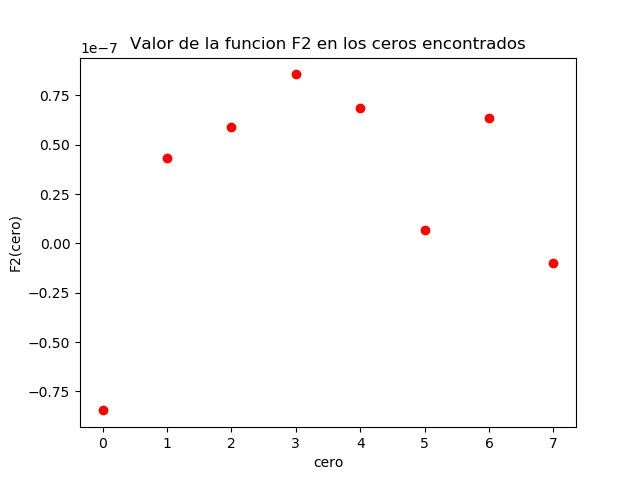
\includegraphics[scale=0.5]{ajuste.png}
\caption{Función $F_2$ evaluada en los ceros encontrados} 
\label{ceros}
\end{figure}

\subsection{Conclusiones y Discusi\'on}

%Se puede apreciar que la función $F_2$ evaluada en los ceros encontrados por \textit{biseccion_modificada()} son del orden de $10^{-8}$ por lo que se considera que el algoritmo logró su objetivo.\\
Se puede apreciar que la función $F_2$ evaluada en los ceros encontrados por textit{biseccion-modificada}  son del orden de $10^{-8}$ por lo que se considera que el algoritmo logró su objetivo.\\
Al utilizar algoritmos de tipo siempre existe la posibilidad de que no se pueda llegar al resultado exacto debido a que pueden ser necesarios infinitos pasos para que converja, o bien, la representación discreta de los números reales no incluye la respuesta esperada.\\ 
En este caso se resolvieron funciones del estilo $\Re^2 \rightarrow \Re$ por lo que fue posible graficar las funciones para encontrar los valores de a y b que inician el proceso de la bisección, lamentablemente para funciones de mayor dimensión no será posible repetir esta metodología ya que no es posible graficar funciones de muchas dimensiones en una pantalla.\\
\textbf{Bonus:} 'In the beginning the Universe was created. This has made a lot of
people very angry and been widely regarded as a bad move.' -- Douglas Adam. \\
Para encontrar el bonus se entró a GitHub Desktop y se buscó en el commit del 27/09 11:58, el mensaje apareció en la descripción del commit.

\end{document}
